% !TEX root = ../main.tex

\clearpage
% Source PDF page 59.
\section{第一版后记}

好的，本书到此结束\textasciitilde{}

欢迎各高校的奶龙同好会分享本书、使用本书作为社团教材。本书为纯开源乐子书籍，欢迎各位奶家人以本校的奶蛙活动为基础进行教材版本的更新与补充。

鄙人们奶疏学浅，本书关于奶蛙的知识如有错误，请您谅解！

% !TEX root = ../../main.tex
\begin{figure}[H]
  \centering
  \phantomsection
  \addcontentsline{lof}{figure}{\protect\numberline{}后记插图: 我的梦想}
  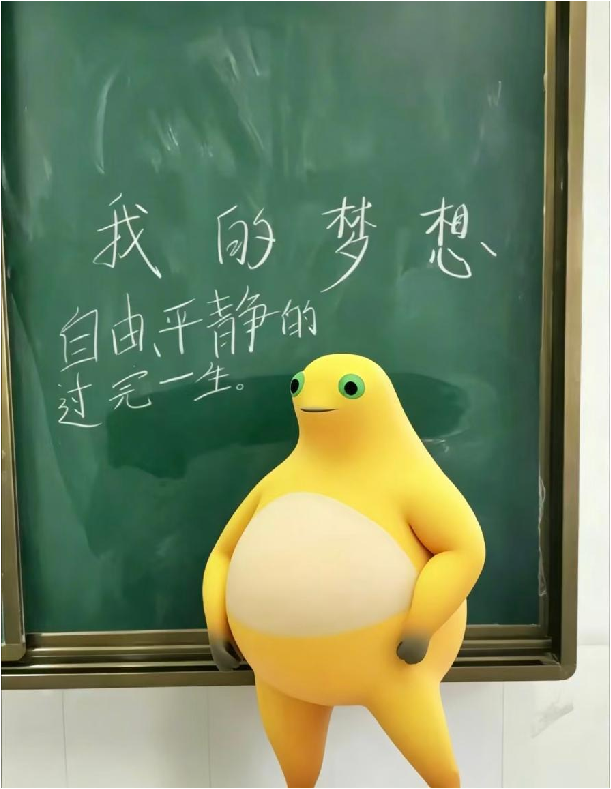
\includegraphics[width=249.12bp,height=0.76\textheight,keepaspectratio]{figures/afterword/afterword.pdf}
\end{figure}


下为一些有趣的奶蛙网站：

\begingroup
\small
\noindent \url{https://www.naiwa.world/}\quad 奶蛙档案局\par
\noindent \url{https://github.com/timerring/codex-pet-naiwa}\quad Codex-奶蛙桌宠\par
\noindent \url{https://github.com/Ensurezwwyyds/tokenbaby}\quad Codex-ChatGPT 额度奶蛙倒数器\par
\noindent \url{https://yhsome.github.io/BigNaiWa}\quad 合成大奶蛙\par
\noindent \url{https://66970010-boop.github.io/frog-miner/}\quad 黄金奶工\par
\noindent \url{https://milkyfrog.com/games}\quad 奶蛙游戏大合集（含数十款经典新奇奶蛙游戏！）\par
\endgroup

\begin{flushright}
\bfseries
《捧腹大笑思想与奶龙学概论（第一版）》编写组\par
Tono\_Hanna、Chishoo、Tachibana\_Sherry
\end{flushright}

